\documentclass[a4paper,11pt]{report}
%
%--------------------   start of the 'preamble'
%
\usepackage{graphicx,amssymb}  %% ... with default font
%\usepackage{graphicx,amssymb,mathptmx}  %%% times roman font
%\usepackage{graphicx,amssymb,mathpazo}   %%% another font
%\usepackage{graphicx,amssymb,newcent}   %%% another font
%\usepackage{graphicx,amssymb,cmbright}   %% yet another
%%%%%%%%%     more fonts in Chap 7 of the 'Companion'
%
\newcommand\etc{\textsl{etc}}
\newcommand\eg{\textsl{eg.}\ }
\newcommand\etal{{\em et al.}}
\newcommand\Quote[1]{\lq\textsl{#1}\rq}
\newcommand\fr[2]{{\textstyle\frac{#1}{#2}}}
%
%---------------------   end of the 'preamble'
%
\begin{document}
%-----------------------------------------------------------
\title{{\tt TetGen}\\ Develop Document}
\author{Hang Si}
\maketitle
%-----------------------------------------------------------
\begin{abstract}\centering
This document is about the implementations of {\tt TetGen}.
\end{abstract}
%-----------------------------------------------------------
\tableofcontents
%-----------------------------------------------------------
\chapter{Mesh Data Structure}
\label{chap:meshds}

Let $\Omega$ be a three-dimensional domain with boundary $\partial\Omega$. A tetrahedral mesh of $\Omega$ is a three-dimensional simplicial complex ${\cal T}$. It contains a subcomplex ${\cal F}$ which is the surface mesh of $\partial\Omega$. ${\cal F}$ a two-dimensional simplicial complex.

For storing and maintaining a tetrahedral mesh ${\cal T}$ as well as its subcomplex ${\cal F}$, we use the following lists of elements:
\begin{itemize}
\item a list of vertices of ${\cal T}$;
\item a list of tetrahedra of ${\cal T}$;
\item a list of subfaces of ${\cal F}$; and
\item a list of subsegment of ${\cal F}$.
\end{itemize}
Where subfaces and subsegments are those faces and edges belong to both ${\cal T}$ and {\cal F}, respectively. Since we store all tetrahedra, there is no need to store faces and edges of ${\cal T}$. While subfaces and subsegments are stored explicitly. 

\section{Basic Mesh Data Types}

There are four types of mesh elements: vertices, tetrahedra, subfaces, and subsegments. The elements of all the four types consist of a tetrahedral mesh of a 3D domain.  Three data structures are declared:  {\it tetrahedron}, {\it shellface}, and {\it point}. A tetrahedron is a tetrahedron;  a shellface can be either a subface or a subsegment;  and a point is a point. These three data types, linked by pointers comprise a mesh.

\subsection{Point}

The {\it point} data structure is a list of floating-point numbers. This list contains the following data of the point:
\begin{itemize}
\item $3$ coordinates;
\item $n$ user-defined attributes (optional);
\item $1$ user-defined metric tensor (optional);
\item $1$ pointer to a simplex (tet, tri, edge); 
\item $1$ pointer to a parent (or duplicate) point;
\item $1$ pointer to a tet in background mesh (optional);
\item $1$ integer index (also for boundary marker);
\item $1$ integer for the vertex type.
\end{itemize}

\subsection{Shellface}

The {\it shellface} data structure represents either a subface or a subsegment. It contains the following data (see Fig.~\ref{fig:shellface-tetrahedron} left):
\begin{itemize}
\item $3$ pointers to adjacent subfaces;
\item $3$ pointers to its points;
\item $2$ pointers to adjacent tetrahedra;
\item $3$ pointers to adjacent subsegments;
\item $1$ pointer to a badface (optional);
\item $1$ double of maximum area (optional);
\item $1$ integer of boundary marker;
\item $1$ integer of type;
\end{itemize}

Fig.~\ref{fig:shellface} shows a subface with its adjacent subfaces, subsegments, and tetrahedra. Note that the three adjacent subsegments is not always exist, if so, they are set to {\tt dummysh}). 

\begin{figure}
  \centering
  \includegraphics[width=0.6\textwidth]{../figs/triang-edge-ds}
\caption{The shellface data structures.}
\label{fig:shellface}
\end{figure}

Note that a shellface is also used to store a subsegment. In such case, the third point of it is set to {\tt null}. And it has only one pointer to an adjacent subface.  Since there may be arbitrary number of subfaces containing a subsegment, chose one arbitrarily.

\subsection{Tetrahedron}

The {\it tetrahedron} data structure represent a tetrahedron. It contains the following data (see Fig.~\ref{fig:tetrahedron} right):
\begin{itemize}
\item $4$ pointers to adjacent tetrahedron;
\item $4$ pointers to its points;
\item $4$ pointers to adjacent subfaces (optional, -p, -r options);
\item $2$ pointers to adjacent subsegments (optional, -p, -r options);
\item $n$ user-defined attributes (optional);
\item $1$ double of maximum volume (optional);
\item $1$ pointer to a list of higher order nodes (-o2 option);
\end{itemize}

\begin{figure}
  \centering
  \includegraphics[width=0.8\textwidth]{../figs/tetrahedron-based}
\caption{The tetrahedron data structures.}
\label{fig:tetrahedron}
\end{figure}

\section{Mesh Handles}

Two special data types, 'triface' and 'face' are defined for maintaining and updating meshes. They are like pointers (or handles), which allow you to hold one particular part of the mesh, i.e., a tetrahedron, a triangle, an edge and a vertex.  However, these data types do not themselves store any part of the mesh. The mesh is made of the data types defined above.

\subsection{Face}

Let the three vertices of a triangle be ordered and numbered as $v_0$, $v_1$, and $v_2$. The six versions of the directed edges $(i, j)$ of this triangle (see Fig.~\ref{fig:edge-versions}) are defined as follows:\\
\begin{tabular}{rl}
$0$ & $(v_0, v_1)$\\
$1$ & $(v_1, v_0)$\\
$2$ & $(v_1, v_2)$\\
$3$ & $(v_2, v_1)$\\
$4$ & $(v_2, v_0)$\\
$5$ & $(v_0, v_2)$
\end{tabular}\\
The {\it face} handle holds a directed edge of a shellface. A set of mesh manipulation primitives are defined for various operation on faces.

\begin{figure}
  \centering
  \includegraphics[width=1.0\textwidth]{../figs/face-versions}
\caption{The six versions of the directed edges of a triangle.}
\label{fig:edge-versions}
\end{figure}

\subsection{Triface}

Let the four nodes of a tetrahedron be ordered and numbered from $v_0, ..., v_3$. The order of the nodes is chosen in such a way that the signed volume of the tetrahedron evaluated by $v_0, ..., v_3$ is negative. Intuitively, the last node ($v_3$) "sees" the first three nodes ($v_0, v_1, v_2$) in counterclockwise order. 

Let the four faces of a tetrahedron be numbered from $f_0, ..., f_3$.  Each face has $6$ directed edges (edge versions are the same as in Fig.~\ref{fig:edge-versions}). We stipulate the four faces and the directed edges in each face as in Fig.~\ref{fig:triface}.

\begin{figure}
  \centering
  \begin{tabular}{cc}
  \includegraphics[width=0.45\textwidth]{../figs/triface-f0} &
  \includegraphics[width=0.45\textwidth]{../figs/triface-f1} \\
  $f_0: (v_0, v_1, v_2)$ & $f_1: (v_0, v_3, v_1)$\\
  \includegraphics[width=0.45\textwidth]{../figs/triface-f2} &
  \includegraphics[width=0.45\textwidth]{../figs/triface-f3} \\
  $f_2: (v_1, v_3, v_2)$ & $f_3: (v_2, v_3, v_0)$
  \end{tabular}
\caption{The faces and directed edges of a tetrahedron.}
\label{fig:triface}
\end{figure}
 
The {\it triface} handle holds a directed edge of a terahedron. A set of mesh manipulation primitives are defined for various operation on trifaces.

\section{Primitives for Mesh Manipulations}

The mesh data structures additionally store geometric informations which help for fast queries.

\subsection{bond}

Suppose two trifaces $t_1$ and $t_2$ share the same faces. The {\tt bond} primitive connects $t_1$ and $t_2$ together. It also encodes the $0$-th edge informations of $t_1$ and $t_2$, i.e., at $t_1$ side, the edge of $t_2$ which corresponding to the $0$-th edge of $t_1$ is bonded, and vice versa at $t_2$ side.

\begin{figure}
  \centering
  \includegraphics[width=1.0\textwidth]{../figs/fnext-base}
\caption{The {\tt bond()} and {\tt fnext()} primitives.}
\label{fig:fnext}
\end{figure}

For an example, in Fig.~\ref{fig:fnext} left, let $t_1$ be the bottom shaded face, and $t_2$ be the top shaded face. Then $t_1$ connects to the $4$-th edge of $t_2$, and $t_2$ connects the $4$-th edge of $t_1$.

\subsection{fnext}

Let $t_1$ be a triface representing the tetrahedron $(v_0, v_1, v_2, v_3)$, and $t_1$ also represents the face $(v_0, v_1, v2)$ (see Fig.~\ref{fig:fnext}), and it holds the edge $[v_0, v_1]$. The {\tt fnext} primitive returns a new triface $t_2$ such that $t_2$ holds the same edge $[v_0, v_1]$, and it represents a face $v_0, v_1, v_k]$ which is the next face in the face ring of the edge $[v_0, v_1]$, and $t_1$, $t_2$ represent different tetrahedra, respectively. 


\chapter{Mesh Transformations}

Mesh transformation operations translate an old set of tetrahedra into a new set of tetrahedra in the same region of the tetrahedralization. Such operations include face/edge flips, vertex insertion/deletions.

\section{Point insertion}

This section discusses the implementation of inserting a vertex. The Bowyer-Watson algorithm~\cite{Bowyer81, Watson81} is used to implement this. It also handles the insertion of hull vertex, i.e., the convex hull will be updated.

\begin{figure}
  \centering
  \includegraphics[width=0.9\textwidth]{../figs/bowyerwatson1}
\caption{Insert a interior vertex. Here {\tt insertpt} lies inside the convex hull.}
\label{fig:bowyerwatson1}
\end{figure}

\begin{figure}
  \centering
  \includegraphics[width=0.6\textwidth]{../figs/inserthullvertex}
\caption{Insert a hull vertex. Here {\tt insertpt} lies outside the convex hull. }
\label{fig:inserthullvertex}
\end{figure}

\begin{figure}
  \centering
  \includegraphics[width=1.0\textwidth]{../figs/bowyerwatson2}
\caption{Insert a hull vertex. Here {\tt insertpt} lies outside the convex hull. {\tt cavetet} is a hull tet, and it points to a side face whose apex is the {\tt dummypoint}. A {\tt newtet} is created on the base face of {\tt cavetet}, it is a hull tet.}
\label{fig:bowyerwatson2}
\end{figure}

\begin{figure}
  \centering
  \includegraphics[width=1.0\textwidth]{../figs/bowyerwatson3}
\caption{Insert a hull vertex. Here {\tt insertpt} lies outside the convex hull. {\tt cavetet} is a hull tet, and it points to its base face which is visible by {\tt insertp}. A {\tt newtet} is created on the base face of {\tt cavetet}, it is not a hull tet.}
\label{bowyerwatson3}
\end{figure}

\section{Primitive Flips}

Given $5$ vertices, denoted ${\bf a}$, ${\bf b}$, ${\bf c}$, ${\bf d}$, and ${\bf e}$, in convex position. There are two primitives flips on these $5$ vertices, which are:
\begin{itemize}
\item {\tt flip23}: transform $2$ tetrahedra to $3$ tetrahedra. As a result, an internal face has been removed and a new edge is inserted.
\item {\tt flip32}: the reverse of {\tt flip23}.
\end{itemize}

\begin{figure}
  \centering
  \includegraphics[width=0.5\textwidth]{../figs/flip-cosph5-2tets}
\caption{Flip operations: 2-to-3 and 3-to-2 flips.}
\label{fig:flip23}
\end{figure}



\chapter{Symbolic Perturbation for {\tt insphere} Test}

This chapter describes a simple symbolic perturbation method for the {\tt insphere} test, so that we can assume there are no five points in $\mathbb{R}^3$ share a common circumscribed sphere. 

\section{The {\tt orient3d} Test}

Let ${\bf a}, {\bf b}, {\bf c}$ be three non-collinear points in $\mathbb{R}^3$.  Let $H$ be the unique plane passing through ${\bf a}$, ${\bf b}$, and ${\bf c}$. We use the {\it left-hand rule} to define the orientation of $H$, i.e., make a fist using your left hand, let the fingers follow the orientation of the sequence $\{{\bf a}$, ${\bf b}$, ${\bf c}\}$, now the half space at the direction of your thumb is defined as the {\it positive open half space} at $H$, denoted as $\mathbb{H}^+$, the other half space is defined as the {\it negative open half space} at $H$, denoted as $\mathbb{H}^-$, see figure~\ref{fig:orient3d}.

\begin{figure}
\centering{
\includegraphics[width=0.6\textwidth]{../figs/orient3d}
}
\caption{The orientation of the plane $H$.}
\label{fig:orient3d}
\end{figure}

Let ${\bf d} \in \mathbb{R}^3$ be a fourth point. The {\tt orient3d} test is defined as follows
\begin{equation}
  \textrm{orient3d}({\bf a}, {\bf b}, {\bf c}, {\bf d})
  \left\{
  \begin{array}{ccl}
  > & 0, & \textrm{if ${\bf d}$ lies in $\mathbb{H}^+$},\\
  = & 0, & \textrm{if ${\bf d}$ lies on $H$},\\
  < & 0, & \textrm{if ${\bf d}$ lies in $\mathbb{H}^-$}.  
  \end{array}
  \right.
\end{equation}
Geometrically, the plane $H$ has the equation
\[
 n_x x + n_y y + n_z z + d = 0,
\]
where $(n_x, n_y, n_z)$ is a unit normal on $H$ and $d$ is the negative of the offset of $H$ from the origin. Every point in $H$ (such as ${\bf a}$, ${\bf b}$ and ${\bf c}$) must satisfy the plane equation. The points in $\mathbb{H}^+$ must satisfy the equation
\[
 n_x x + n_y y + n_z z + d > 0.
\]
Hence the points in $\mathbb{H}^+$ are those points in $\mathbb{R}^3$ which lie "above" $H$. Similarly, the points on $\mathbb{H}^-$ are those points  in $\mathbb{R}^3$ which lie "below" $H$. Note that the terms "above" and "below" are relative to the normal of $H$.

Finally, it is well-known that the {\tt orient3d} test on four points can be calculated by taking the sign of the determinat of the matrix of their homogenous coordinates, i.e.,
\begin{equation}
  \textrm{orient3d}({\bf a}, {\bf b}, {\bf c}, {\bf d}) = \textrm{det}({\bf A}).
\end{equation}
where ${\bf A}$ is a $4 \times 4$ matrix
\[
  {\bf A} = \left[\begin{array}{cccc}
      a_x & a_y & a_z & 1\\
      b_x & b_y & b_z  & 1\\
      c_x & c_y & c_z  & 1\\
      d_x & d_y & d_z  & 1
      \end{array}\right].
\]
Geometrically, $\textrm{orient3d}({\bf a}, {\bf b}, {\bf c}, {\bf d})$ is $6$ times of the signed volume of the tetrahedron ${\bf abcd}$.

\section{The {\tt insphere} Test}

Let ${\bf a}, {\bf b}, {\bf c}, {\bf d}$ be four non-coplanar points in $\mathbb{R}^3$ and ${\bf e} \in \mathbb{R}^3$ be a fifth point.% and they form a positive orientation, i.e., $a, b, c$ follow the fingers of your left-hand's fist with thumb pointing to $d$. 
Let $\Sigma$ be the unique circumscribed sphere passing through the four points. The {\tt insphere} test is defined as follows
\begin{equation}
  \textrm{insphere}({\bf a}, {\bf b}, {\bf c}, {\bf d}, {\bf e})
  \left\{
  \begin{array}{ccl}
  > & 0, & \textrm{if ${\bf e}$ lies inside $\Sigma$},\\
  = & 0, & \textrm{if ${\bf e}$ lies on $\Sigma$},\\
  < & 0, & \textrm{if ${\bf e}$ lies outside $\Sigma$}.  
  \end{array}
  \right.
\end{equation}
It is well known that such test can be computed in the following way:
\begin{equation}\label{equ:insph}
 \textrm{insphere}({\bf a}, {\bf b}, {\bf c}, {\bf d}, {\bf e}) = \frac{\textrm{det}({\bf A})}{\textrm{sign}(\textrm{orient3d}({\bf a}, {\bf b}, {\bf c}, {\bf d}))},
\end{equation}
where ${\bf A}$ is a $5 \times 5$ matrix
\begin{equation}
  {\bf A} = \left[\begin{array}{ccccc}
      a_x & a_y & a_z & a_l & 1\\
      b_x & b_y & b_z & b_l & 1\\
      c_x & c_y & c_z & c_l & 1\\
      d_x & d_y & d_z & d_l & 1\\
      e_x & e_y & e_z & e_l & 1 
      \end{array}\right].
\end{equation}
In the above, $a_l$ is obtained from the coordinates of $a$ by,
$a_l = a_x^2 + a_y^2 + a_z^2$.  The same for $b_l$, $c_l$, and $d_l$. $\textrm{sign}(x)$ is the sign function, i.e., it returns one of $\{1, 0, -1\}$ depending on $x$ is large than, equal, or less than $0$, respectively.

Geometrically, the {\tt insphere} test in $\mathbb{R}^3$ can be seen as an orientation test in $\mathbb{R}^4$ if there is a {\it lifting map} $\omega: \mathbb{R}^3 \to \mathbb{R}^4$ such that for each point ${\bf s} = (s_x, s_y, s_z)$ of $\mathbb{R}^3$ $\omega({\bf s}) = (s_x, s_y, s_z, s_l)$ of $\mathbb{R}^4$ with $s_l = s_x^2 + s_y^2 + s_z^2$.  The return value of the {\tt insphere} test is the $4! = 24$ times of the signed volume of the $4$-dimensional simplex ${\bf abcde}$. 

\section{Symbolic Perturbation}

Five points in $\mathbb{R}^3$ have a common circumscribed sphere if and only if their images by $\omega$ lie in a hypeplane of $\mathbb{R}^4$. The symbolic perturbation of the {\tt insphere} test consists in adding respectively some value to the fourth coordinate of $\omega({\bf a}), \omega({\bf b}), \omega({\bf c}), \omega({\bf d}), \omega({\bf e})$ so that these points are not in the same hyperplane any more in $\mathbb{R}^4$. Then the predicate answers positive or negative instead of zero.

Let $S$ be a finite set of $n$ points be ordered like $\{{\bf s}_1, {\bf s}_2, {\bf s}_3, ... {\bf s}_{n}\}$ in $\mathbb{R}^3$. For each point ${\bf s} \in S$, we perturb it by adding a perturbation in $\omega({\bf s})$ by
\begin{equation}
\omega({\bf s}) = (s_{x}, s_{y}, s_{z}, s_{l}-s_{w}),
\end{equation}
where $s_w$ is an infinitesimal and $s_w > 0$. The quantity of the perturbation will determine the final result of the {\tt insphere} test. We will discuss it at the end of this section.

Now assume ${\bf a}, {\bf b}, {\bf c}, {\bf d}, {\bf e}$ lie on a common circumscribed sphere, i.e., $\textrm{det}({\bf A}) = 0$. We re-compute the {\tt insphere} test by using the five perturbed points $\omega({\bf a}), \omega({\bf b}), \omega({\bf c}), \omega({\bf d}), \omega({\bf e})$, i.e., 
\[
  \textrm{insphere}(\omega({\bf a}), \omega({\bf b}), \omega({\bf c}), \omega({\bf d}), \omega({\bf e})) = \frac{\textrm{det}({\bf A}^{\omega})}{\textrm{sign}\left(\textrm{orient3d}({\bf a}, {\bf b}, {\bf c}, {\bf d})\right)}
\]
Where
\begin{equation}
  {\bf A}^{\omega} = \left[\begin{array}{ccccc}
      a_x & a_y & a_z & a_l - a_w & 1\\
      b_x & b_y & b_z & b_l - b_w & 1\\
      c_x & c_y & c_z & c_l - c_w & 1\\
      d_x & d_y & d_z & d_l - d_w & 1\\
      e_x & e_y & e_z & e_l - e_w & 1 
      \end{array}\right].
\end{equation}

Since the determinant is a linear function and by the assumption that ${\bf a}$, ${\bf b}$, ${\bf c}$, ${\bf d}$, and ${\bf e}$ are co-spherical. We can compute $\textrm{det}({\bf A}^{\omega})$ by
\[
  \begin{array}{rcccl}
  \textrm{det}({\bf A}^{\omega}) 
   &=& \textrm{det}\left(
      \left[\begin{array}{ccccc}
      a_x & a_y & a_z & a_l & 1\\
      b_x & b_y & b_z & b_l & 1\\
      c_x & c_y & c_z & c_l & 1\\
      d_x & d_y & d_z & d_l & 1\\
      e_x & e_y & e_z & e_l & 1 
      \end{array}\right]\right) &+& 
      \textrm{det}\left(
      \left[\begin{array}{ccccc}
      a_x & a_y & a_z & 1 & a_w\\
      b_x & b_y & b_z & 1 & b_w\\
      c_x & c_y & c_z & 1 & c_w\\
      d_x & d_y & d_z & 1 & d_w\\
      e_x & e_y & e_z & 1 & e_w
      \end{array}\right]\right)\\
    &=& 0 &+& \textrm{det}\left(
      \left[\begin{array}{ccccc}
      a_x & a_y & a_z & 1 & a_w\\
      b_x & b_y & b_z & 1 & b_w\\
      c_x & c_y & c_z & 1 & c_w\\
      d_x & d_y & d_z & 1 & d_w\\
      e_x & e_y & e_z & 1 & e_w
      \end{array}\right]\right).\\
  \end{array}
\]
Expand the above determinant along the last column\footnote{The determinant formula
\[
  \textrm{det}({\bf A}) = \sum_{j=1}^{n} (-1)^{i+j} a_{ij} {\bf M}_{ij}({\bf A}),
\]
where ${\bf A}$ is a $n \times n$ matrix, ${\bf M}_{ij}(a)$ (called the {\it $(i,j)$ minor} of $a$) is the determinant of the $(n-1) \times (n-1)$ submatrix of ${\bf A}$ formed by deleting $i$-th row and $j$-th column of $a$.}, we get
\begin{equation}\label{equ:perturb}
  \textrm{det}({\bf A}^{\omega}) = a_w \textrm{det}({\bf A}_a) - b_w \textrm{det}({\bf A}_b) + c_w \textrm{det}({\bf A}_c) - d_w \textrm{det}({\bf A}_d) + e_w \textrm{det}({\bf A}_e).
\end{equation}
where
\[
  \begin{array}{ccccc}
  \textrm{det}({\bf A}_a) &=& \textrm{det}\left(\left[\begin{array}{cccc}
              b_x & b_y & b_z & 1\\
              c_x & c_y & c_z & 1\\
              d_x & d_y & d_z & 1\\
              e_x & e_y & e_z & 1 
              \end{array}\right]\right) 
              &=& \textrm{orient3d}({\bf b}, {\bf c}, {\bf d}, {\bf e});\\ 
   \textrm{det}({\bf A}_b) &=& \textrm{det}\left(\left[\begin{array}{cccc}
               a_x & a_y & a_z & 1\\
               c_x & c_y & c_z & 1\\
               d_x & d_y & d_z & 1\\
               e_x & e_y & e_z & 1 
               \end{array}\right]\right)
              &=& \textrm{orient3d}({\bf a}, {\bf c}, {\bf d}, {\bf e});\\
    \textrm{det}({\bf A}_c) &=& \textrm{det}\left(\left[\begin{array}{cccc}
                a_x & a_y & a_z & 1\\
                b_x & b_y & b_z & 1\\
                d_x & d_y & d_z & 1\\
                e_x & e_y & e_z & 1 
                \end{array}\right]\right)
               &=& \textrm{orient3d}({\bf a}, {\bf b}, {\bf d}, {\bf e});\\ 
     \textrm{det}({\bf A}_d) &=& \textrm{det}\left(\left[\begin{array}{cccc}
                 a_x & a_y & a_z & 1\\
                 b_x & b_y & b_z & 1\\
                 c_x & c_y & c_z & 1\\
                 e_x & e_y & e_z & 1 
                 \end{array}\right]\right)
               &=& \textrm{orient3d}({\bf a}, {\bf b}, {\bf c}, {\bf e});\\
      \textrm{det}({\bf A}_e) &=& \textrm{det}\left(\left[\begin{array}{cccc}
                  a_x & a_y & a_z & 1\\
                  b_x & b_y & b_z & 1\\
                  c_x & c_y & c_z & 1\\
                  d_x & d_y & d_z & 1
                  \end{array}\right]\right)
               &=& \textrm{orient3d}({\bf a}, {\bf b}, {\bf c}, {\bf d}).
  \end{array}
\]

Since we assume that the four points ${\bf a}$, ${\bf b}$, ${\bf c}$, and ${\bf d}$ are non-coplanar, hence $\textrm{det}({\bf A}_e) \neq 0$. Moreover, this assumption implies that there are at most one determinant in $\textrm{det}({\bf A}_a), ..., \textrm{det}({\bf A}_d)$ can be zero, otherwise, ${\bf a}$, ${\bf b}$, ${\bf c}$, and ${\bf d}$ would be coplanar. It is possible to let $\textrm{det}({\bf A}^{\omega})$ not be zero by appropriate choosing the perturbations $a_w, ..., e_w$.

A simple strategy is to choose such a perturbations i to let $a_w >> b_w >> c_w >> d_w >> e_w$. Then the sign of $\textrm{det}({\bf A}^{\omega})$ is determined by the first non-zero determinant in the right hand side of (\ref{equ:perturb}).

One way to implement the above strategy is to use the index of the points, i.e., {\it the one with smaller index gets bigger perturbation than the one with higher index}.

\section{Examples}

This section gives few examples to illustrate how the perturbation technique of the above section work.  In the following examples, let ${\bf a}, {\bf b}, {\bf c}, {\bf d}, {\bf e}$ are points in $\mathbb{R}^3$ and their indices are in increasing order.

\begin{figure}
\centering{
\includegraphics[width=0.8\textwidth]{../figs/symbolicperturb1}
}
\caption{Symbolic perturbation. The five points ${\bf a}, {\bf b}, {\bf c}, {\bf d}, {\bf e}$ share a circumscribed sphere.}
\label{fig:ex1}
\end{figure}

The first example (see Figure~\ref{fig:ex1}) is in the case which no four points are coplanar. The two pictures show the same five points but the labeling of points are different.  In the left figure, let's evaluate $\textrm{insphere}({\bf a}, {\bf b}, {\bf c}, {\bf e}, {\bf d})$ with their perturbed points. Since
\[
\begin{array}{rcl}
\textrm{det}({\bf A}^{\omega}) &=& 
a_w\textrm{orient3d}({\bf b}, {\bf c}, {\bf e}, {\bf d})\\
& & -b_w\textrm{orient3d}({\bf a}, {\bf c}, {\bf e}, {\bf d})\\
& & +c_w\textrm{orient3d}({\bf a}, {\bf b}, {\bf e}, {\bf d})\\
& & -e_w\textrm{orient3d}({\bf a}, {\bf b}, {\bf c}, {\bf d})\\
& & +d_w\textrm{orient3d}({\bf a}, {\bf b}, {\bf c}, {\bf e})\\
&\approx& a_w\textrm{orient3d}({\bf b}, {\bf c}, {\bf e}, {\bf d})
\end{array}
\]
Then
\[
\begin{array}{rcl}
\textrm{insphere}({\bf a}, {\bf b}, {\bf c}, {\bf e}, {\bf d}) &=&
\frac{\textrm{det}({\bf A}^{\omega})}{\textrm{sign}(\textrm{orient3d}({\bf a}, {\bf b}, {\bf c}, {\bf e}))}\\
&=& \frac{a_w\textrm{orient3d}({\bf b}, {\bf c}, {\bf e}, {\bf d})}{\textrm{sign}\left(\textrm{orient3d}({\bf a}, {\bf b}, {\bf c}, {\bf e})\right)}\\
&<& 0.
\end{array}
\]
It shows that the tetrahedron ${\bf abce}$ is Delaunay. Next we evaluate $\textrm{insphere}({\bf e}, {\bf d}, {\bf b}, {\bf a}, {\bf c})$ in the left figure. Since
\[
\begin{array}{rcl}
\textrm{det}({\bf A}^{\omega}) &=& 
e_w\textrm{orient3d}({\bf d}, {\bf b}, {\bf a}, {\bf c})\\
& & -d_w\textrm{orient3d}({\bf e}, {\bf b}, {\bf a}, {\bf c})\\
& & +b_w\textrm{orient3d}({\bf e}, {\bf d}, {\bf a}, {\bf c})\\
& & -a_w\textrm{orient3d}({\bf e}, {\bf d}, {\bf b}, {\bf c})\\
& & +c_w\textrm{orient3d}({\bf e}, {\bf d}, {\bf b}, {\bf a})\\
&\approx& -a_w\textrm{orient3d}({\bf e}, {\bf d}, {\bf b}, {\bf c})
\end{array}
\]
Then
\[
\begin{array}{rcl}
\textrm{insphere}({\bf e}, {\bf d}, {\bf b}, {\bf a}, {\bf c}) &=&
\frac{\textrm{det}({\bf A}^{\omega})}{\textrm{sign}\left(\textrm{orient3d}({\bf e}, {\bf d}, {\bf b}, {\bf a})\right)}\\
&=& \frac{-a_w\textrm{orient3d}({\bf e}, {\bf d}, {\bf b}, {\bf c})}{\textrm{sign}\left(\textrm{orient3d}({\bf e}, {\bf d}, {\bf b}, {\bf a})\right)}\\
&>& 0
\end{array}
\]
It shows that the tetrahedron ${\bf edba}$ is non-Delaunay. Both tests are consistent (no contradiction).  The right figure has the same set of vertices as the left but different labeling (indices) of the vertices. Hence the Delaunay tetrahedra are different as the left. The check is left as an exercise.\\*

\begin{figure}
\centering{
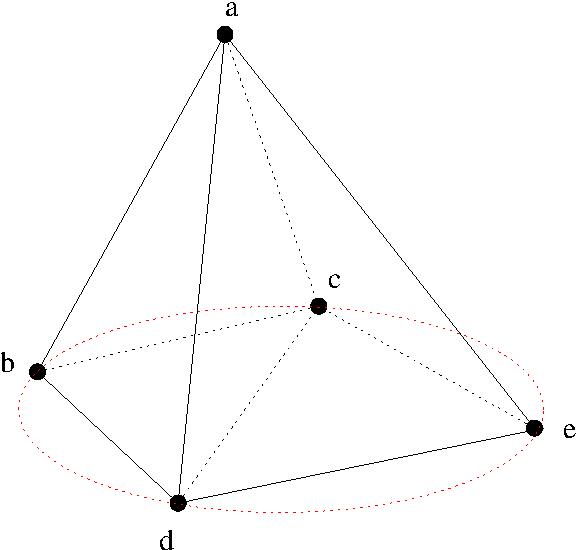
\includegraphics[width=0.4\textwidth]{../figs/symbolicperturb2}
}
\caption{Symbolic perturbation of five coplanar points. In this example, four point are coplanar.}
\label{fig:ex2}
\end{figure}

The second example (see Fig.~\ref{fig:ex2}) illustrates the case which four points ${\bf b}, {\bf c}, {\bf d}, {\bf e}$ are both coplanar and cospherical. Let's evaluate $\textrm{insphere}({\bf d},{\bf c},{\bf a},{\bf b},{\bf e})$ in its perturbed case. Since
\[
\begin{array}{rcl}
\textrm{det}({\bf A}^{\omega}) &=&
d_w\textrm{orient3d}({\bf c},{\bf a},{\bf b},{\bf e})\\
& & -c_w\textrm{orient3d}({\bf d},{\bf a},{\bf b},{\bf e})\\
& & +a_w\textrm{orient3d}({\bf d},{\bf c},{\bf b},{\bf e})\\
& & -b_w\textrm{orient3d}({\bf d},{\bf c},{\bf a},{\bf e})\\
& & +e_w\textrm{orient3d}({\bf d},{\bf c},{\bf a},{\bf b})\\
&\approx& +a_w\textrm{orient3d}({\bf d},{\bf c},{\bf b},{\bf e})\\
& & -b_w\textrm{orient3d}({\bf d},{\bf c},{\bf a},{\bf e})\\
&=& -b_w\textrm{orient3d}({\bf d},{\bf c},{\bf a},{\bf e})
\end{array}
\]
Then
\[
\begin{array}{rcl}
\textrm{insphere}({\bf d},{\bf c},{\bf a},{\bf b},{\bf e}) &=&
\frac{\textrm{det}({\bf A}^{\omega})}{\textrm{sign}\left(\textrm{orient3d}({\bf d},{\bf c},{\bf a},{\bf b})\right)}\\
&=& \frac{-b_w\textrm{orient3d}({\bf d},{\bf c},{\bf a},{\bf e})}{\textrm{sign}\left(\textrm{orient3d}({\bf d},{\bf c},{\bf a},{\bf b})\right)}\\
&>& 0
\end{array}
\]

Next let evaluate $\textrm{insphere}({\bf b},{\bf e},{\bf a},{\bf c},{\bf d})$ in its perturbed case. Since
\[
\begin{array}{rcl}
\textrm{det}({\bf A}^{\omega}) &=&
b_w\textrm{orient3d}({\bf e},{\bf a},{\bf c},{\bf d})\\
& & -e_w\textrm{orient3d}({\bf b},{\bf a},{\bf c},{\bf d})\\
& & +a_w\textrm{orient3d}({\bf b},{\bf e},{\bf c},{\bf d})\\
& & -c_w\textrm{orient3d}({\bf b},{\bf e},{\bf a},{\bf d})\\
& & +d_w\textrm{orient3d}({\bf b},{\bf e},{\bf a},{\bf c})\\
&\approx& +a_w\textrm{orient3d}({\bf b},{\bf e},{\bf c},{\bf d})\\
& & +b_w\textrm{orient3d}({\bf e},{\bf a},{\bf c},{\bf d})\\
&=& b_w\textrm{orient3d}({\bf e},{\bf a},{\bf c},{\bf d})
\end{array}
\]
Then
\[
\begin{array}{rcl}
\textrm{insphere}({\bf b},{\bf e},{\bf a},{\bf c},{\bf d}) &=&
\frac{\textrm{det}({\bf A}^{\omega})}{\textrm{sign}\left(\textrm{orient3d}({\bf b},{\bf e},{\bf a},{\bf c})\right)}\\
&=& \frac{b_w\textrm{orient3d}({\bf e},{\bf a},{\bf c},{\bf d})}{\textrm{sign}\left(\textrm{orient3d}({\bf b},{\bf e},{\bf a},{\bf c})\right)}\\
&<& 0
\end{array}
\]

The tests show that the two tetrahedra containing edge ${\bf cd}$ are non-Delaunay, while the two containing edge ${\bf be}$ are Delaunay, which are consistent. 

\section{The {\tt insphere\_sos} Test}

In this section, we implement a {\tt insphere} test which returns only either a positive or negative value, no zero. Define
\begin{equation}
  \textrm{insphere\_sos}({\bf a}, {\bf b}, {\bf c}, {\bf d}, {\bf e})
  \left\{
  \begin{array}{ccl}
  > & 0, & \textrm{if ${\bf e}$ lies inside the circumsphere of ${\bf abcd}$},\\
  < & 0, & \textrm{if ${\bf e}$ lies outside the circumsphere of ${\bf abcd}$}.  
  \end{array}
  \right.
\end{equation}

The algorithm is listed below. The input assumption is that the tetrahedron ${\bf abcd}$ is not degenerate, i.e., its volume is not zero.

\begin{figure}[h]
\begin{tabular}{l}
{\tt REAL} {\sc inspshere\_sos}(${\bf a}$, ${\bf b}$, ${\bf c}$, ${\bf d}$, ${\bf e}$)\\
// The input points ${\bf a}$, ${\bf b}$, ${\bf c}$, and ${\bf d}$ are non-coplanar.
\end{tabular}\\
\begin{tabular}{rl}
$1$ & {\tt ori} = $\textrm{orient3d}({\bf a}, {\bf b}, {\bf c}, {\bf d})$; // assert({\tt ori} $\neq$ 0);\\ 
$2$ & {\tt sign} = $\textrm{insphere}({\bf a}, {\bf b}, {\bf c}, {\bf d}, {\bf e})$;\\
$3$ & {\bf if} {\tt sign} $\neq$ 0 {\bf then}\\
$4$ & $\quad$ {\bf if} {\tt ori} $<$ 0 {\bf then} {\tt sign} = -{\tt sign}; {\bf endif}\\
$5$ & $\quad$ {\bf return} {\tt sign};\\
$6$ & {\bf endif}\\
 & // Symbolic perturbation.\\
$7$ & sort the input sequence $\{ {\bf a}, {\bf b}, {\bf c}, {\bf d}, {\bf e}\}$ according to  the increasing order\\
 & of their indices;\\
 & Let the new sequence of the five points be $\{\alpha, \beta, \gamma, \delta, \epsilon\}$.\\
 & Let ${\tt swaps}$ be the number of position switches between the two sequences.\\
$8$ & {\tt oriA} = $\textrm{orient3d}(\beta, \gamma, \delta, \epsilon)$;\\
$9$ & {\bf if} {\tt oriA} $\neq$ 0 {\bf then}\\
$10$ & $\quad$ {\bf if} ${\tt swaps}$ is odd {\bf then} {\tt oriA} = -{\tt oriA}; {\bf endif}\\
$11$ & $\quad$ {\bf if} {\tt ori} $<$ 0 {\bf then} {\tt oriA} = -{\tt oriA}; {\bf endif}\\
$12$ & $\quad$ return {\tt oriA};\\
$13$ & {\bf endif}\\
$14$ & {\tt oriB} = -$\textrm{orient3d}(\alpha, \gamma, \delta, \epsilon)$; // assert({\tt oriB} $\neq$ 0)\\
$15$ & {\bf if} ${\tt swaps}$ is odd {\bf then} {\tt oriB} = -{\tt oriB}; {\bf endif}\\
$16$ & {\bf if} {\tt ori} $<$ 0 {\bf then} {\tt oriB} = -{\tt oriB}; {\bf endif}\\
$17$ & return {\tt oriB};\\
\end{tabular}
\end{figure}

This algorithm assumes that we don't know the orientation of the point sequence ${\bf a}$, ${\bf b}$, ${\bf c}$, and ${\bf d}$. In our implementation of Delaunay algorithm, we actually know the positive orientation of any tetrahedron. Hence we can speed up the test by giving the positive sequence for ${\bf a}$, ${\bf b}$, ${\bf c}$, and ${\bf d}$. Hence {\tt ori} $>$ 0. So the lines $1, 4, 11, 16$ can be skipped.

%-----------------------------------------------------------
\addcontentsline{toc}{chapter}{\numberline{}Bibliography}
\include{biblio}
%-----------------------------------------------------------
\end{document}
